\chapter{Analyse}

%Baggrund. Referere til et Link på nettet hvor praktik rapporten ligger.
Responsum K/S er en virksomhed der besvarer andre virksomheders opkald, som en ekstern reception. For at kunne dette gør de brug af telefonanlæg, databaser og PC baserede klienter. Deres nuværende system er udviklet tilbage i 90'erne og består for en stor del af komponenter der ikke længere udvikles på, og derfor efterhånden slæber rundt på en del fejl og mangler. Som følge heraf gik Adaheads K/S igang med at udvikle et fremtidssikret open source system baseret på GPL licensen for at sikre, at koden altid er tilgængelig for systemets brugere.

Responsum K/S har behov for at kunne lave kaldplaner til at modtage og dirigere opkald til henholdsvis receptionister eller automatiske systemer som IVR menuer og telefonsvarer. Der skal knyttes information til alle indgående opkald, sådan at receptionister og systemer kan håndtere dem korrekt. For at kunne oprette og vedligholde kaldplaner og virksomhedsinformation skal der være administrative værktøjer til rådighed.

\pagebreak

\section{Oversigt}
AdaHeads' produkt består af følgende systemer:
\begin{figure}[ht!]
\centering
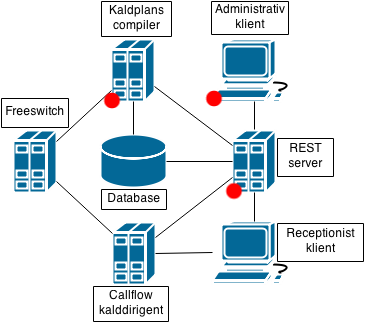
\includegraphics[scale=0.5]{images/adaheads_system.png}
\caption{En oversigt over Adaheads system.}
\label{fig:adaheadssystem}
\end{figure}
\begin{enumerate}
	\item{Freeswitch PBX til håndtering af opkald} 
	\item{Kaldplan-compiler til generering af Freeswitch XML kaldplaner}
	\item{Administrativ browser baseret klient til interaktion med REST interfaces}
	\item{Relationel database}
	\item{REST intefaces, fordelt på flere HTTP servere}
	\item{CallFlow kald dirigenten håndterer kaldrelateret kommunikation mellem Freeswitch og resten af systemet}
	\item{Browser baseret klient til receptionister}
\end{enumerate}
Komponenterne markeret med rød er designet og konstrueret i dette projekt
%Linjen skal være på samme side som figuren.

\pagebreak

\section{Kravspecifikation}
Kravene er formuleret i samarbejde med kunden og tager hensyn til tidshorisonten på projektet, den tekniske kompleksitet og kundens behov.

\paragraph{Funktionelle krav}
\begin{enumerate}
  \item[F01.] Brug af interfaces kræver bruger autentificering
  \item[F02.] Man skal kunne oprette, ændre og slette organisationer
  \item[F03.] Man skal kunne oprette, ændre og slette receptioner
  \item[F04.] Man skal kunne oprette, ændre og slette kontaktpersoner
  \item[F05.] Man skal kunne tilføje og fjerne en kontaktpersons relation til en reception
  \item[F06.] Man skal kunne ændre en kontaktpersons data relativt til en reception
  \item[F07.] Man skal kunne oprette og opdatere kaldplaner
  \item[F08.] Man skal kunne tilknytte en kommentar til alle komponenter i en kaldplan
  \item[F09.] Man skal kunne viderestille indgående opkald til arbitrære telefonnumre
  \item[F10.] Man skal kunne afspille en lydfil for opkalder til af velkomsthilsner og lignende
  \item[F11.] Man skal kunne sende opkald til receptionisterne
  \item[F12.] Man skal kunne sende opkald til en IVR menu
  \item[F13.] Man skal kunne sende opkald til telefonsvarer
  \item[F14.] Man skal kunne dirigere opkald på basis af tid
  \item[F15.] En kaldplan skal kunne tilknyttes Freeswitch
\end{enumerate}

\paragraph{Non-Funktionelle krav}
\begin{enumerate}
  \item[NF1.] Al server software skal være kompatibelt med Linux og/eller *BSD
  \item[NF2.] Klienten skal køre i en browser
  \item[NF3.] Koden skal være GPL licenseret
\end{enumerate}

\section{Use case}
For at få en fornemmelse for, hvor kravene bliver brugt henne og om man har overset noget er det en god ide, at lave use case\citep{LarmanUml}.
Mange operationer på serveren, er klassiske CRUD (Create, Read, Update, Delete) operationer. Den første use case kan med små ændringer dække over de første 4 krav.


\section{Opret reception}
Følgende senariere kan også finde sted for organizationer og kontaktpersoner i receptioner.

\begin{table}[h]
    \begin{tabular}{|p{3cm}|p{8.3cm}|}
    \hline
    Formål         & At oprette en ny reception til en organisation                              \\ \hline
    Succestilstand & Receptionen bliver oprettet og gemt i databasen.                            \\ \hline
    Fejltilstand   & Der bliver ikke oprettet nogen receptionen, og brugeren 
                     får en fejlmeddelelse. \\ \hline
    Aktør          & Serviceagent                                                                \\ \hline
    \end{tabular}
\end{table}

\begin{enumerate}
  \item Login med tilstrækkelig rettigheder.
  \begin{enumerate}
    \item Hvis brugeren ikke har noget login eller ikke har tilstrækkelige rettigheder. Sendes brugeren ud til login vinduet igen.
  \end{enumerate}
  \item Tryk på "ny reception" knappen.
  \item Indtast informationen den nye reception skal have.
  \item Tryk gem. Derved bliver der sendt en forespørgsel til serveren om at oprette en ny reception.
  \begin{enumerate}
    \item Hvis brugeren har indtastet ugyldig informationen eller har mistet forbindelsen til serveren, får brugeren at vide at der er sket en fejl.
  \end{enumerate}
\end{enumerate}

%\section{Ændre reception}
%\begin{enumerate}
%  \item Login med tilstrækkelig rettigheder.
%  \item Vælg den rette reception.
%  \item Tilret information.
%  \item Tryk på gem, og information bliver updateret i systemet.
%\end{enumerate}

%\section{Slet reception}
%\begin{enumerate}
%    \item Login med tilstrækkelig rettigheder.
%    \item vælg den rette reception.
%    \item Tryk på slet, hvilket sletter reception på serveren.
%\end{enumerate}

%\section{Aktivere reception}
%\begin{enumerate}
%    \item Login med tilstrækkelig rettigheder.
%    \item vælg den deaktiveret reception.
%    \item Tryk på aktivere, hvilket aktivere reception på serveren igen.
%\end{enumerate}

\section{Dialplan}
\begin{table}[h]
    \begin{tabular}{|p{3cm}|p{8.3cm}|}
    \hline
    Formål         & At ændre en receptions dialplan                              \\ \hline
    Succestilstand & Dialplanen er ændret og ligger klar i databasen, til at compileren henter den.                         \\ \hline
    Fejltilstand   & Der bliver ikke gemt nogen ændringer, og bruger får en fejl meddelelse. \\ \hline
    Aktør          & Serviceagent                                                                \\ \hline
    \end{tabular}
\end{table}

\begin{enumerate}
    \item Login med tilstrækkelig rettigheder.
  \begin{enumerate}
    \item Hvis brugeren ikke har noget login eller ikke har tilstrækkelige rettigheder. Sendes brugeren ud til login vinduet igen.
  \end{enumerate}
    \item Vælg receptionen.
    \item Begynd og redigere dens dialplan.
    \item Tryk gem og ændringerne bliver sendt til serveren der gemmer det i databasen.
  \begin{enumerate}
    \item Hvis brugeren har indtastet ugyldig informationen eller har mistet forbindelsen til serveren, får brugeren at vide at der er sket en fejl.
  \end{enumerate}
\end{enumerate}